% =====================================================================
%  Chapitre 1 -- Fondements du machine learning (2 h)
%  Introduction au Machine Learning -- CNFSDP -- L3 S5 -- 2026-2027
%  Version niveau licence (12/10/2026)
%  Compilation : pdflatex chapitre1.tex (deux fois)
% =====================================================================
\documentclass[aspectratio=169,11pt]{beamer}
\usetheme{CNFSDP}
\usetikzlibrary{positioning,arrows.meta}
\usepackage{colortbl}

\chapitre{1}
\chapitrecourt{Ch.~1 \textendash{} Fondements}

\title{Chapitre 1 \textendash{} Fondements du machine learning}
\subtitle{Prédire, mesurer l'erreur, éviter le sur-apprentissage}
\author{Rois Céti DIMBAMBA}
\institute{Ingénieur statisticien économiste \textperiodcentered{} Actuaire \textperiodcentered{} \href{https://rdimbamba.shinyapps.io/roisceti_e-cv/}{\textcolor{cnfVert}{CV en ligne}}}
\date{14 octobre 2026}

\begin{document}

% ---------------------------------------------------------------------
\begin{frame}[plain,noframenumbering]
  \titlepage
\end{frame}

\begin{frame}{Plan et objectifs}
  \begin{columns}[T]
    \begin{column}{0.44\textwidth}
      \footnotesize\tableofcontents
    \end{column}
    \begin{column}{0.54\textwidth}
      \begin{objectifs}
        \footnotesize
        \begin{itemize}
          \item Savoir ce qu'est un problème d'apprentissage et en connaître le vocabulaire.
          \item Définir l'erreur d'un modèle : perte, risque, risque empirique.
          \item Connaître le meilleur prédicteur possible et l'erreur irréductible.
          \item Comprendre le sur-apprentissage et la bonne façon d'évaluer un modèle.
          \item Lire les métriques usuelles : RMSE, précision, rappel, AUC.
        \end{itemize}
      \end{objectifs}
      \vskip-1mm{\scriptsize\color{cnfGris}Prérequis : chapitre~0 (espérance, variance, probabilité conditionnelle).}
    \end{column}
  \end{columns}
\end{frame}

% =====================================================================
\section{Qu'est-ce que le machine learning ?}

\begin{frame}{Apprendre à partir d'exemples}
  \begin{definition}[Machine learning, ou apprentissage automatique]
    Ensemble de méthodes qui construisent \emph{automatiquement}, à partir d'exemples observés, une règle permettant de prédire ou de résumer des données nouvelles.
  \end{definition}
  \begin{columns}[T]
    \begin{column}{0.48\textwidth}
      \textbf{Programmation classique}\\[1mm]
      {\small On écrit la règle à la main : « si la mère a fait le secondaire et vit en ville, alors l'enfant est vacciné ».}
    \end{column}
    \begin{column}{0.48\textwidth}
      \textbf{Machine learning}\\[1mm]
      {\small On fournit des milliers d'exemples (enfants, caractéristiques, vacciné ou non) ; l'algorithme \emph{apprend} la règle.}
    \end{column}
  \end{columns}
  \vskip3mm
  \begin{exemple}
    Prédire le revenu d'un ménage, la vaccination complète d'un enfant, le défaut de remboursement d'un emprunteur ; regrouper des ménages qui se ressemblent.
  \end{exemple}
\end{frame}

\begin{frame}{Le tableau de données}
  \begin{columns}[T]
    \begin{column}{0.56\textwidth}
      \small
      \renewcommand{\arraystretch}{1.2}
      \begin{tabular}{c|ccc|c}
        & \multicolumn{3}{c|}{variables explicatives $x$} & cible $y$ \\
        enfant & âge mère & éducation & milieu & vacciné \\ \hline
        1 & 24 & primaire & rural & 0 \\
        2 & 31 & secondaire & urbain & 1 \\
        3 & 19 & aucune & rural & 0 \\
        4 & 28 & secondaire & rural & 1 \\
        $\vdots$ & $\vdots$ & $\vdots$ & $\vdots$ & $\vdots$
      \end{tabular}
    \end{column}
    \begin{column}{0.42\textwidth}
      \small
      \begin{itemize}
        \item Une \textbf{ligne} = un individu $i=1,\dots,n$.
        \item Les \textbf{variables explicatives} de l'individu $i$ forment un vecteur $x_i\in\R^d$.
        \item La \textbf{variable cible} $y_i$ est ce que l'on veut prédire.
        \item Les $x_i$ forment une matrice $X$ à $n$ lignes et $d$ colonnes.
      \end{itemize}
    \end{column}
  \end{columns}
  \vskip3mm
  {\small\color{cnfGris}Les variables qualitatives (éducation, milieu) sont codées en nombres avant l'apprentissage (chapitre~5).}
\end{frame}

\begin{frame}{Les grandes familles de problèmes}
  \centering
  \begin{tikzpicture}[
      every node/.style={align=center,execute at begin node={\hyphenpenalty=10000\exhyphenpenalty=10000}},
      racine/.style={fill=cnfVert,text=white,rounded corners=1.5mm,inner sep=2mm,font=\bfseries},
      famille/.style={draw=cnfVert,fill=cnfVertPale,rounded corners=1.5mm,inner sep=1.6mm,text width=3.5cm,minimum height=1.25cm,anchor=north,font=\small},
      horsprog/.style={draw=cnfGris!50,fill=cnfGrisClair,text=cnfGris,rounded corners=1.5mm,inner sep=1.6mm,text width=2.45cm,minimum height=1.25cm,anchor=north,font=\small},
      tache/.style={draw=cnfGris!45,fill=white,rounded corners=1mm,inner sep=1.4mm,text width=2.55cm,minimum height=2.1cm,anchor=north,font=\footnotesize},
      lien/.style={-{Stealth[length=1.8mm]},draw=cnfGris,semithick}]
    \node[racine] (ml) at (0.4,0) {Machine learning};
    \node[famille] (sup) at (-4.2,-0.85) {\textbf{Supervisé}\\on observe des couples $(x_i,y_i)$};
    \node[famille] (nsup) at (2.2,-0.85) {\textbf{Non supervisé}\\on observe seulement les $x_i$};
    \node[horsprog] (renf) at (5.95,-0.85) {\textbf{Renforcement}\\hors programme};
    \draw[lien] (ml.south) -- (sup.north); \draw[lien] (ml.south) -- (nsup.north); \draw[lien] (ml.south) -- (renf.north);
    \node[tache] (reg) at (-5.7,-2.75) {\textbf{Régression}\\[0.5mm]$y\in\R$\\ex. : revenu\\[0.5mm]{\color{cnfVert}chapitre~2}};
    \node[tache] (cla) at (-2.7,-2.75) {\textbf{Classification}\\[0.5mm]$y\in\{0,1\}$\\ex. : vacciné ?\\[0.5mm]{\color{cnfVert}chapitre~3}};
    \node[tache] (dim) at (0.7,-2.75) {\textbf{Réduction de dimension}\\[0.5mm]ACP\\ex. : indice de richesse\\[0.5mm]{\color{cnfVert}chapitre~4}};
    \node[tache] (clu) at (3.7,-2.75) {\textbf{Classification non supervisée}\\[0.5mm]k-means, CAH\\ex. : typologie de ménages\\[0.5mm]{\color{cnfVert}chapitre~4}};
    \draw[lien] (sup.south) -- (reg.north); \draw[lien] (sup.south) -- (cla.north);
    \draw[lien] (nsup.south) -- (dim.north); \draw[lien] (nsup.south) -- (clu.north);
  \end{tikzpicture}
  \vskip2mm
  {\small\color{cnfGris}Ce chapitre pose le cadre du supervisé ; le non supervisé a son propre cadre au chapitre~4.}
\end{frame}

% =====================================================================
\section{Formaliser la prédiction}

\begin{frame}{Données et prédicteur}
  \begin{definition}[Données]
    On note $X$ le vecteur des variables explicatives et $Y$ la variable cible d'un individu tiré au hasard dans la population : $(X,Y)$ est un couple \emph{aléatoire}, dont la loi est \emph{inconnue}.
    On dispose d'un \emph{échantillon d'apprentissage} $\Dn=\{(x_1,y_1),\dots,(x_n,y_n)\}$ : $n$ réalisations indépendantes de $(X,Y)$.
  \end{definition}
  \begin{definition}[Prédicteur]
    Un \emph{prédicteur} est une fonction $f$ qui, à des caractéristiques $x$, associe une prédiction $f(x)$ de $y$.
    Un \emph{algorithme d'apprentissage} fabrique un prédicteur $\hat f$ à partir de l'échantillon $\Dn$.
  \end{definition}
  \begin{remarque}
    Le prédicteur appris dépend de l'échantillon : avec une autre enquête, on obtiendrait un $\hat f$ un peu différent.
  \end{remarque}
\end{frame}

\begin{frame}{Mesurer une erreur : la fonction de perte}
  \begin{definition}[Perte]
    Une \emph{perte} est une fonction $\ell(\hat y,y)\ge0$ qui mesure le coût de prédire $\hat y$ quand la vraie valeur est $y$.
  \end{definition}
  \vskip1mm
  \begin{center}
    \renewcommand{\arraystretch}{1.35}
    \begin{tabular}{llll}
      \toprule
      \textbf{Perte} & \textbf{Formule} & \textbf{Usage} & \textbf{Exemple} \\
      \midrule
      quadratique & $\ell(\hat y,y)=(\hat y-y)^2$ & régression & prédit $3$, vrai $5$ : perte $4$ \\
      absolue & $\ell(\hat y,y)=|\hat y-y|$ & régression & prédit $3$, vrai $5$ : perte $2$ \\
      0-1 & $\ell(\hat y,y)=\begin{cases}1&\text{si }\hat y\ne y\\0&\text{sinon}\end{cases}$ & classification & prédit $1$, vrai $0$ : perte $1$ \\
      \bottomrule
    \end{tabular}
  \end{center}
  \vskip1mm
  {\small\color{cnfGris}La perte quadratique pénalise fortement les grosses erreurs ; la perte absolue est moins sensible aux valeurs extrêmes.}
\end{frame}

\begin{frame}{Risque et risque empirique}
  \begin{definition}[Risque, risque empirique]
    Le \emph{risque} d'un prédicteur $f$ est son erreur moyenne sur toute la population :
    \[
      R(f)=\E\big[\ell\big(f(X),Y\big)\big].
    \]
    Son \emph{risque empirique} est son erreur moyenne sur l'échantillon :
    \[
      \Rn(f)=\frac1n\sum_{i=1}^n\ell\big(f(x_i),y_i\big).
    \]
  \end{definition}
  \begin{itemize}\small
    \item En classification avec la perte 0-1, $R(f)=\P\big(f(X)\ne Y\big)$ : la \emph{probabilité d'erreur}.
    \item Le risque est l'objectif, mais il est inconnu (la loi de $(X,Y)$ l'est) ; le risque empirique, lui, se calcule.
    \item Si $f$ est fixé à l'avance, la loi des grands nombres donne $\Rn(f)\approx R(f)$ pour $n$ grand.
  \end{itemize}
\end{frame}

\begin{frame}{Un calcul de risque empirique}
  \small
  On veut prédire le nombre d'enfants $y$ d'une femme selon son milieu $x$ (urbain, rural), sur $n=10$ femmes :
  urbain : $2,3,2,3$ ; rural : $4,5,3,6,5,4$.
  \vskip2mm
  \begin{columns}[T]
    \begin{column}{0.48\textwidth}
      \textbf{Prédicteur constant} $f_0(x)=\bar y=3{,}7$ :
      \[
        \Rn(f_0)=\tfrac{1}{10}\textstyle\sum_i(y_i-3{,}7)^2=1{,}61 .
      \]
    \end{column}
    \begin{column}{0.48\textwidth}
      \textbf{Prédicteur par milieu} : moyenne de chaque groupe,
      $f_1(\text{urbain})=2{,}5$, $f_1(\text{rural})=4{,}5$ :
      \[
        \Rn(f_1)=\tfrac{1}{10}\,(1+5{,}5)=0{,}65 .
      \]
    \end{column}
  \end{columns}
  \vskip3mm
  \begin{remarque}[Lecture]
    Utiliser l'information $x$ divise l'erreur quadratique moyenne par plus de deux.
    Le prédicteur $f_1$ prédit, dans chaque groupe, la moyenne du groupe : c'est exactement le meilleur prédicteur de la section suivante.
  \end{remarque}
\end{frame}

% =====================================================================
\section{Le meilleur prédicteur possible}

\begin{frame}{La meilleure constante est la moyenne}
  \begin{proposition}
    Soit $Z$ une variable aléatoire de variance finie. Pour tout réel $c$,
    \[
      \E\big[(Z-c)^2\big]=\Var(Z)+\big(\E[Z]-c\big)^2 .
    \]
    La fonction $c\mapsto\E\big[(Z-c)^2\big]$ atteint donc son minimum en $c=\E[Z]$, et la valeur minimale est $\Var(Z)$.
  \end{proposition}
  \begin{preuve}
    On écrit $Z-c=(Z-\E Z)+(\E Z-c)$ et l'on développe le carré :
    $\E[(Z-c)^2]=\E[(Z-\E Z)^2]+2(\E Z-c)\,\E[Z-\E Z]+(\E Z-c)^2$.
    Le terme du milieu est nul car $\E[Z-\E Z]=0$.
  \end{preuve}
  \begin{remarque}[Lecture]
    Si l'on doit résumer une variable par un seul nombre et que l'on paie le carré de l'erreur, il faut choisir sa moyenne ; l'erreur restante est sa variance.
  \end{remarque}
\end{frame}

\begin{frame}{Régression : le meilleur prédicteur est la moyenne conditionnelle}
  \begin{theoreme}[Prédicteur de Bayes en régression]
    En perte quadratique, le prédicteur qui a le plus petit risque est
    \[
      f^*(x)=\E[Y\mid X=x],
    \]
    la moyenne de $Y$ parmi les individus ayant les caractéristiques $x$. On l'appelle \emph{prédicteur de Bayes}.
  \end{theoreme}
  \begin{preuve}[(idée)]
    Pour chaque valeur $x$, on doit choisir un nombre $f(x)$ qui prédit $Y$ dans le groupe des individus tels que $X=x$.
    La proposition précédente, appliquée à la loi de $Y$ dans ce groupe, dit que le meilleur choix est la moyenne du groupe, $\E[Y\mid X=x]$.
  \end{preuve}
  \begin{remarque}
    En perte absolue, le même raisonnement donne la \emph{médiane} de $Y$ dans chaque groupe (admis) : plus robuste pour des revenus très dispersés.
  \end{remarque}
\end{frame}

\begin{frame}{L'erreur irréductible}
  \begin{definition}[Risque de Bayes, excès de risque]
    Le \emph{risque de Bayes} $R^*=R(f^*)$ est le plus petit risque possible. L'\emph{excès de risque} d'un prédicteur $f$ est $R(f)-R^*\ge0$.
  \end{definition}
  \begin{exemple}[Modèle signal + bruit]
    Si $Y=g(X)+\varepsilon$, où le bruit $\varepsilon$ est indépendant de $X$, de moyenne $0$ et de variance $\sigma^2$, alors
    \[
      f^*(x)=g(x)\qquad\text{et}\qquad R^*=\sigma^2 .
    \]
    Même en connaissant parfaitement $g$, on se trompe en moyenne de $\sigma^2$ : c'est le bruit, que les variables $X$ n'expliquent pas.
  \end{exemple}
  \begin{aretenir}
    Aucun algorithme ne fait mieux que $R^*$. On juge un modèle à la distance entre son risque et $R^*$.
  \end{aretenir}
\end{frame}

\begin{frame}{Classification : le classifieur de Bayes}
  Ici $y\in\{0,1\}$, perte 0-1, et l'on note $\eta(x)=\P(Y=1\mid X=x)$ la probabilité d'être dans la classe $1$ sachant $x$.
  \begin{theoreme}[Classifieur de Bayes]
    Le classifieur qui a la plus petite probabilité d'erreur est
    \[
      f^*(x)=\begin{cases}1&\text{si }\eta(x)>\frac12,\\0&\text{sinon,}\end{cases}
      \qquad\text{et}\qquad R^*=\E\big[\min\{\eta(X),1-\eta(X)\}\big].
    \]
  \end{theoreme}
  \begin{preuve}
    Pour un individu de caractéristiques $x$, prédire $1$ est faux avec probabilité $1-\eta(x)$, prédire $0$ est faux avec probabilité $\eta(x)$.
    La meilleure décision choisit la plus petite des deux, soit $\min\{\eta(x),1-\eta(x)\}$ ; on fait la moyenne sur $X$.
  \end{preuve}
  {\small\color{cnfGris}En clair : on prédit la classe la plus probable sachant ce que l'on observe.}
\end{frame}

\begin{frame}{Un exemple chiffré}
  \small
  $Y=1$ si l'enfant est complètement vacciné, $X$ = niveau d'éducation de la mère (chiffres fictifs).
  \vskip1mm
  \begin{center}
    \renewcommand{\arraystretch}{1.3}
    \begin{tabular}{lccc}
      \toprule
      $x$ & aucune & primaire & secondaire ou plus \\
      \midrule
      $\P(X=x)$ & $0{,}3$ & $0{,}4$ & $0{,}3$ \\
      $\eta(x)=\P(Y=1\mid X=x)$ & $0{,}45$ & $0{,}60$ & $0{,}80$ \\
      $f^*(x)$ & $0$ & $1$ & $1$ \\
      erreur $\min\{\eta(x),1-\eta(x)\}$ & $0{,}45$ & $0{,}40$ & $0{,}20$ \\
      \bottomrule
    \end{tabular}
  \end{center}
  \[
    R^*=0{,}3\times0{,}45+0{,}4\times0{,}40+0{,}3\times0{,}20=0{,}355 .
  \]
  \begin{remarque}[Lecture]
    Avec la seule éducation de la mère, aucun modèle ne peut se tromper moins de $35{,}5\,\%$ du temps. Pour faire mieux, il faut d'autres variables.
  \end{remarque}
\end{frame}

\begin{frame}{Un exemple continu : deux nuages gaussiens}
  \begin{columns}[T]
    \begin{column}{0.54\textwidth}
      \small
      Deux classes équiprobables ; sachant $Y=0$, $X\sim\mathcal N\big((0,0),I_2\big)$ ; sachant $Y=1$, $X\sim\mathcal N\big((1{,}5;1{,}5),I_2\big)$.
      \begin{proposition}[admise]
        Le classifieur de Bayes prédit $1$ si et seulement si $x_1+x_2>1{,}5$ : la frontière est une \emph{droite}.
        Son erreur vaut $R^*=\Phi(-1{,}06)\approx0{,}144$, où $\Phi$ est la fonction de répartition de $\mathcal N(0,1)$.
      \end{proposition}
      \begin{remarque}[Lecture]
        Les nuages se recouvrent : environ $14\,\%$ d'erreurs sont inévitables. Nous comparerons nos modèles à ce plancher.
      \end{remarque}
    \end{column}
    \begin{column}{0.44\textwidth}
      \centering
      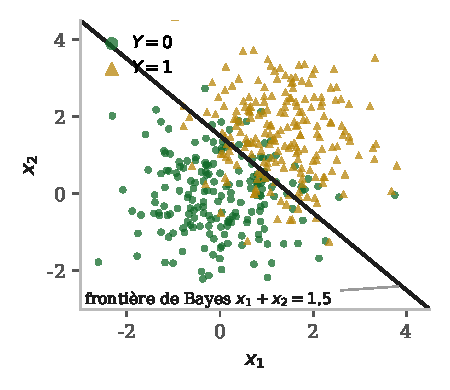
\includegraphics[width=\textwidth]{melange.pdf}
    \end{column}
  \end{columns}
\end{frame}

\begin{frame}{Quand les erreurs n'ont pas le même coût}
  \begin{columns}[T]
    \begin{column}{0.55\textwidth}
      En dépistage, manquer un malade (faux négatif) est plus grave qu'une fausse alerte (faux positif).
      \vskip2mm
      Si un faux négatif coûte $c_{\mathrm{FN}}$ et un faux positif $c_{\mathrm{FP}}$, la règle optimale devient
      \[
        f^*(x)=1\iff\eta(x)>t^*=\frac{c_{\mathrm{FP}}}{c_{\mathrm{FP}}+c_{\mathrm{FN}}} .
      \]
    \end{column}
    \begin{column}{0.42\textwidth}
      \begin{exemple}
        Si manquer un malade coûte $9$ fois plus qu'une fausse alerte : $t^*=\frac{1}{1+9}=0{,}1$.
        On déclare positif dès que la probabilité dépasse $10\,\%$.
      \end{exemple}
    \end{column}
  \end{columns}
  \vskip2mm
  {\small\color{cnfGris}Le seuil $\frac12$ n'est que le cas de coûts égaux.}
\end{frame}

% =====================================================================
\section{Sur-apprentissage}

\begin{frame}{Apprendre, c'est minimiser l'erreur sur l'échantillon}
  \begin{definition}[Minimisation du risque empirique]
    On choisit une famille de prédicteurs $\F$, puis on retient le prédicteur de $\F$ qui fait le moins d'erreurs sur l'échantillon :
    \[
      \hat f\in\argmin_{f\in\F}\Rn(f).
    \]
  \end{definition}
  {\small Exemples de familles : droites ou plans (régression linéaire, chapitre~2) ; arbres de décision de profondeur au plus $p$ (chapitre~3).}
  \vskip2mm
  \begin{columns}[T]
    \begin{column}{0.48\textwidth}
      \begin{remarque}[Famille trop pauvre]
        Elle ne contient pas de bon prédicteur : on se trompe même sur l'échantillon (\emph{sous-apprentissage}).
      \end{remarque}
    \end{column}
    \begin{column}{0.48\textwidth}
      \begin{remarque}[Famille trop riche]
        Elle contient un prédicteur qui colle à chaque point, bruit compris (\emph{sur-apprentissage}).
      \end{remarque}
    \end{column}
  \end{columns}
\end{frame}

\begin{frame}{Le sur-apprentissage en image}
  \begin{columns}[c]
    \begin{column}{0.55\textwidth}
      \centering
      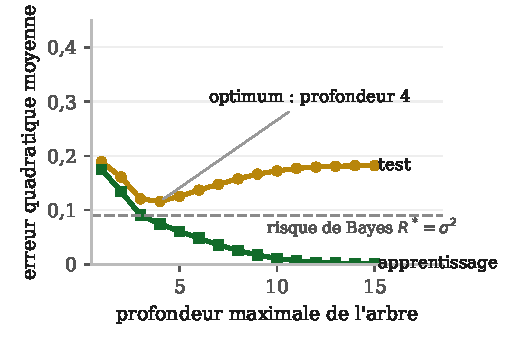
\includegraphics[width=\textwidth]{surapprentissage.pdf}
    \end{column}
    \begin{column}{0.43\textwidth}
      \small
      $Y=\sin(2\pi X)+\varepsilon$, $\sigma=0{,}3$, $n=200$ ; arbres de profondeur $1$ à $15$.
      \begin{itemize}
        \item L'erreur d'apprentissage tend vers $0$ : l'arbre profond \emph{apprend par cœur}, bruit compris.
        \item L'erreur test baisse, puis remonte.
        \item Le meilleur arbre (profondeur $4$) reste au-dessus du plancher $R^*=\sigma^2=0{,}09$.
      \end{itemize}
    \end{column}
  \end{columns}
\end{frame}

\begin{frame}{Biais et variance}
  \small
  En perte quadratique, l'erreur moyenne d'un prédicteur appris se décompose (admis) :
  \[
    \text{erreur test moyenne}=\underbrace{R^*}_{\text{bruit}}+\underbrace{\text{biais}^2}_{\text{modèle trop rigide}}+\underbrace{\text{variance}}_{\text{modèle trop instable}} .
  \]
  \begin{center}
    \renewcommand{\arraystretch}{1.15}
    \begin{tabular}{lll}
      \toprule
      & \textbf{Modèle trop simple} & \textbf{Modèle trop complexe} \\
      \midrule
      Biais & élevé & faible \\
      Variance & faible & élevée \\
      Erreur d'apprentissage & élevée & presque nulle \\
      Diagnostic & sous-apprentissage & sur-apprentissage \\
      \bottomrule
    \end{tabular}
  \end{center}
  \begin{aretenir}
    L'erreur sur les données d'apprentissage est trop optimiste : on n'évalue \alert{jamais} un modèle sur les données qui ont servi à le construire.
  \end{aretenir}
\end{frame}

% =====================================================================
\section{Évaluer et choisir un modèle}

\begin{frame}{Évaluer sur un échantillon test}
  \begin{definition}[Échantillon test, risque test]
    Un \emph{échantillon test} est un ensemble de $m$ individus \emph{non utilisés} pour l'apprentissage. Le \emph{risque test} de $\hat f$ est
    \[
      \widehat R_{\mathrm{test}}(\hat f)=\frac1m\sum_{j=1}^m\ell\big(\hat f(x'_j),y'_j\big).
    \]
  \end{definition}
  Comme $\hat f$ n'a pas vu ces individus, $\widehat R_{\mathrm{test}}$ estime honnêtement le vrai risque.
  \begin{proposition}[Intervalle de confiance d'un taux d'erreur]
    En classification, si $\hat p=\widehat R_{\mathrm{test}}(\hat f)$ est le taux d'erreur sur $m$ individus test, un intervalle de confiance approché à $95\,\%$ pour le vrai taux d'erreur est
    $\hat p\pm1{,}96\sqrt{\hat p(1-\hat p)/m}$ (chapitre~0, théorème central limite).
  \end{proposition}
  {\small\color{cnfGris}Exemple : $\hat p=15\,\%$ sur $m=1\,000$ individus donne $15\,\%\pm2{,}2$ points.}
\end{frame}

\begin{frame}{Apprentissage, validation, test}
  \centering
  \begin{tikzpicture}
    \fill[cnfVert] (0,0) rectangle (7.2,0.8);
    \fill[cnfVertVif!70] (7.2,0) rectangle (9.6,0.8);
    \fill[cnfJaune!80!black] (9.6,0) rectangle (12,0.8);
    \node[text=white,font=\small\bfseries] at (3.6,0.4) {apprentissage ($60\,\%$)};
    \node[text=white,font=\footnotesize\bfseries,align=center] at (8.4,0.4) {validation\\[-0.6mm]($20\,\%$)};
    \node[text=white,font=\footnotesize\bfseries,align=center] at (10.8,0.4) {test\\[-0.6mm]($20\,\%$)};
    \node[font=\footnotesize,text width=6.8cm,align=center] at (3.6,-0.7) {on ajuste chaque modèle candidat};
    \node[font=\footnotesize,text width=2.4cm,align=center] at (8.4,-0.7) {on choisit le meilleur};
    \node[font=\footnotesize,text width=2.4cm,align=center] at (10.8,-0.7) {on mesure, une seule fois};
  \end{tikzpicture}
  \vskip4mm
  \begin{enumerate}
    \item On met de côté un échantillon \textbf{test}, que l'on ne regarde plus jusqu'à la fin.
    \item On ajuste plusieurs modèles sur l'\textbf{apprentissage} et on les compare sur la \textbf{validation}.
    \item On réentraîne le modèle choisi, puis on l'évalue \textbf{une seule fois} sur le test.
  \end{enumerate}
  \begin{remarque}[Fuite d'information]
    Choisir un modèle d'après son score test rend ce score optimiste, comme l'erreur d'apprentissage.
  \end{remarque}
\end{frame}

\begin{frame}{Validation croisée}
  \centering
  \begin{tikzpicture}[x=1.15cm,y=0.42cm]
    \foreach \v in {1,...,5}{
      \foreach \b in {1,...,5}{
        \ifnum\b=\v
          \fill[cnfJaune!80!black] ({\b},{-\v}) rectangle ({\b+0.95},{-\v+0.8});
        \else
          \fill[cnfVert] ({\b},{-\v}) rectangle ({\b+0.95},{-\v+0.8});
        \fi}
      \node[font=\footnotesize,anchor=east] at (0.9,{-\v+0.4}) {tour \v};
      \node[font=\footnotesize,anchor=west] at (6.05,{-\v+0.4}) {erreur $e_\v$};}
    \node[font=\footnotesize] at (3.5,0.6) {les $n$ observations, coupées en $5$ blocs};
  \end{tikzpicture}
  \vskip2mm
  \begin{definition}[Validation croisée à $V$ blocs]
    On coupe l'échantillon en $V$ blocs. À chaque tour, on apprend sur $V-1$ blocs (\textcolor{cnfVert}{vert}) et l'on mesure l'erreur $e_v$ sur le bloc restant (\textcolor{cnfJaune!70!black}{jaune}).
    Le score de validation croisée est la moyenne $\frac1V\sum_{v=1}^Ve_v$.
  \end{definition}
  {\small\color{cnfGris}Chaque observation sert une fois à valider : utile quand les données sont peu nombreuses. En pratique $V=5$ ou $10$.}
\end{frame}

% =====================================================================
\section{Mesurer la performance}

\begin{frame}{Métriques de régression}
  Sur $m$ individus test, avec $\hat y_j$ la prédiction et $y_j$ la vraie valeur :
  \begin{center}
    \renewcommand{\arraystretch}{1.6}
    \begin{tabular}{lll}
      \toprule
      \textbf{Métrique} & \textbf{Formule} & \textbf{Lecture} \\
      \midrule
      EQM (MSE) & $\frac1m\sum_j(\hat y_j-y_j)^2$ & erreur quadratique moyenne \\
      RMSE & $\sqrt{\mathrm{EQM}}$ & même unité que $y$ : « on se trompe d'environ\dots » \\
      MAE & $\frac1m\sum_j|\hat y_j-y_j|$ & erreur absolue moyenne, robuste aux valeurs extrêmes \\
      \bottomrule
    \end{tabular}
  \end{center}
  \begin{exemple}
    Une RMSE de $0{,}9$ enfant signifie qu'on se trompe typiquement d'un peu moins d'un enfant sur le nombre d'enfants d'une femme.
  \end{exemple}
\end{frame}

\begin{frame}{Classification : la matrice de confusion}
  \begin{columns}[T]
    \begin{column}{0.5\textwidth}
      \centering
      \renewcommand{\arraystretch}{1.7}
      \begin{tabular}{r|c|c|}
        \multicolumn{1}{r}{} & \multicolumn{1}{c}{\textbf{prédit 1}} & \multicolumn{1}{c}{\textbf{prédit 0}} \\ \cline{2-3}
        \textbf{vrai 1} & \textbf{VP} $\boldsymbol{=116}$ & FN $=26$ \\ \cline{2-3}
        \textbf{vrai 0} & FP $=18$ & \textbf{VN} $\boldsymbol{=140}$ \\ \cline{2-3}
      \end{tabular}
      \vskip2mm
      \begin{minipage}{0.92\linewidth}\raggedright\scriptsize\color{cnfGris}
        VP : vrais positifs ; FN : faux négatifs ; FP : faux positifs ; VN : vrais négatifs ; $m=300$ individus test.
      \end{minipage}
    \end{column}
    \begin{column}{0.46\textwidth}
      \small
      \begin{itemize}
        \item \textbf{Exactitude} : $\frac{\mathrm{VP}+\mathrm{VN}}{m}=\frac{256}{300}=0{,}853$.
        \item \textbf{Précision} : parmi les prédits positifs, part de vrais positifs, $\frac{\mathrm{VP}}{\mathrm{VP}+\mathrm{FP}}=0{,}866$.
        \item \textbf{Rappel} : parmi les vrais positifs, part détectée, $\frac{\mathrm{VP}}{\mathrm{VP}+\mathrm{FN}}=0{,}817$.
        \item \textbf{F1} : $\frac{2\times\text{précision}\times\text{rappel}}{\text{précision}+\text{rappel}}=0{,}841$.
      \end{itemize}
    \end{column}
  \end{columns}
  \vskip2mm
  \begin{remarque}[Classes déséquilibrées]
    Si $5\,\%$ des enfants sont émaciés, prédire « personne n'est émacié » donne $95\,\%$ d'exactitude\dots{} et un rappel nul.
  \end{remarque}
\end{frame}

\begin{frame}{Scores, courbe ROC et AUC}
  \begin{columns}[T]
    \begin{column}{0.6\textwidth}
      \small
      Beaucoup de modèles donnent un \emph{score} $s(x)$, par exemple une estimation de $\eta(x)$, puis classent en $1$ si $s(x)>t$.
      \begin{definition}[Courbe ROC, AUC]
        Quand le seuil $t$ varie, on trace le taux de vrais positifs (rappel) en fonction du taux de faux positifs ($1-$ spécificité) : c'est la \emph{courbe ROC}.
        L'\emph{AUC} est l'aire sous cette courbe.
      \end{definition}
      \textbf{Interprétation} (admise) : l'AUC est la probabilité qu'un positif tiré au hasard ait un score plus élevé qu'un négatif tiré au hasard.
      $0{,}5$ = hasard, $1$ = classement parfait.
    \end{column}
    \begin{column}{0.38\textwidth}
      \centering
      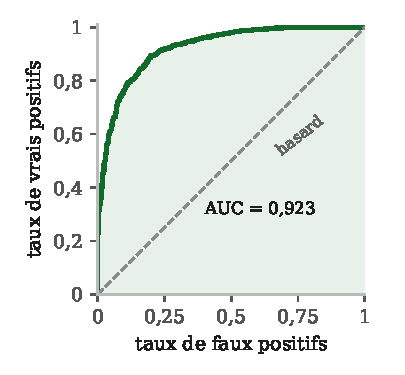
\includegraphics[width=\textwidth]{roc.pdf}
    \end{column}
  \end{columns}
\end{frame}

\begin{frame}{L'outil : scikit-learn}
  \small
  \renewcommand{\arraystretch}{1.25}
  \begin{tabular}{p{0.36\textwidth}p{0.56\textwidth}}
    \toprule
    \textbf{Instruction} & \textbf{Rôle} \\
    \midrule
    \texttt{f.fit(X, y)} & apprend le prédicteur $\hat f$ sur l'échantillon \\
    \texttt{f.predict(X)} & calcule les prédictions $\hat f(x)$ \\
    \texttt{f.predict\_proba(X)[:, 1]} & donne le score $s(x)$, estimation de $\eta(x)$ \\
    \texttt{train\_test\_split} & sépare apprentissage et test \\
    \texttt{cross\_val\_score} & validation croisée \\
    \texttt{GridSearchCV} & choix des réglages par validation croisée \\
    \texttt{sklearn.metrics} & EQM, matrice de confusion, AUC\dots \\
    \bottomrule
  \end{tabular}
  \vskip2mm
  Tous les modèles du cours partagent cette interface : changer de modèle revient à changer une ligne.
\end{frame}

% =====================================================================
\section{En Python}

\begin{frame}[fragile]{Comparer des modèles au classifieur de Bayes}
\begin{python}[basicstyle=\ttfamily\scriptsize]
import numpy as np
from sklearn.linear_model import LogisticRegression
from sklearn.tree import DecisionTreeClassifier
rng = np.random.default_rng(0)

def simuler(n):                                # deux nuages gaussiens
    y = rng.integers(0, 2, n)
    return rng.standard_normal((n, 2)) + 1.5 * y[:, None], y

X, y = simuler(1_000); Xt, yt = simuler(10_000)   # apprentissage, test
m = len(yt)
for nom, f in [("logistique", LogisticRegression()),
               ("arbre profond", DecisionTreeClassifier(random_state=0))]:
    err = np.mean(f.fit(X, y).predict(Xt) != yt)  # taux d'erreur test
    print(nom, round(err, 4), "±", round(1.96 * np.sqrt(err * (1 - err) / m), 4))
print("Bayes", np.mean((Xt.sum(axis=1) > 1.5) != yt))
# logistique 0.1476 ± 0.007 | arbre profond 0.2049 ± 0.0079 | Bayes 0.1445
\end{python}
\vskip-1mm
{\small\color{cnfGris}La logistique est presque au plancher de Bayes ; l'arbre profond sur-apprend.}
\end{frame}

\begin{frame}[fragile]{Validation croisée, matrice de confusion, AUC}
\begin{python}[basicstyle=\ttfamily\scriptsize]
from sklearn.model_selection import cross_val_score
from sklearn.metrics import roc_auc_score, confusion_matrix
y = rng.integers(0, 2, 1_000)
X = rng.standard_normal((1_000, 2)) + 1.5 * y[:, None]

f = LogisticRegression()
print(cross_val_score(f, X, y, cv=5).round(3))  # [0.82 0.88 0.895 0.835 0.87]

f.fit(X[:700], y[:700])                        # 700 pour apprendre, 300 pour tester
s, yt = f.predict_proba(X[700:])[:, 1], y[700:]
print(confusion_matrix(yt, s > 0.5))           # [[VN FP] [FN VP]] = [[140 18] [26 116]]
print(round(roc_auc_score(yt, s), 4))          # 0.9395
\end{python}
\vskip-1mm
{\small\color{cnfGris}Attention : scikit-learn range la matrice avec la classe $0$ en premier, à l'inverse du tableau du cours.}
\end{frame}

% =====================================================================
\section{TP en salle}

\begin{frame}{TP1 \textendash{} Erreur de Bayes, sur-apprentissage, évaluation}
  \footnotesize
  \begin{tp}{TP1 \textendash{} à faire en salle}{30 min \textperiodcentered{} \texttt{notebooks/TP1.ipynb} (Colab)}
    \textbf{Partie A (régression)} : $n=200$ points de $Y=\sin(2\pi X)+\varepsilon$, $\sigma=0{,}3$.
    \begin{enumerate}\setlength\itemsep{0pt}
      \item Ajuster des arbres de profondeur $1$ à $15$ ; tracer les erreurs d'apprentissage et test ; comparer à $\sigma^2$.
      \item Refaire l'apprentissage sur $20$ échantillons tirés avec remise : comparer les arbres de profondeur $15$ et $3$. Lequel varie le plus ?
    \end{enumerate}
    \textbf{Partie B (classification)} : les deux nuages gaussiens du cours.
    \begin{enumerate}\setcounter{enumi}{2}\setlength\itemsep{0pt}
      \item Comparer les taux d'erreur test de la logistique, d'un arbre profond et du classifieur de Bayes ($R^*\approx0{,}144$).
      \item Donner l'intervalle de confiance à $95\,\%$ de chaque taux d'erreur.
      \item Choisir la profondeur d'un arbre par validation croisée ; tracer la courbe ROC et calculer l'AUC.
    \end{enumerate}
  \end{tp}
\end{frame}

\begin{frame}{Résumé}
  \begin{itemize}
    \item Un problème supervisé : prédire $Y$ à partir de $X$, à l'aide d'un échantillon d'exemples.
    \item On mesure l'erreur par une perte ; le risque est l'erreur moyenne sur la population.
    \item Le meilleur prédicteur possible : la moyenne conditionnelle $\E[Y\mid X=x]$ en régression, la classe la plus probable en classification. Son erreur $R^*$ est irréductible.
    \item Un modèle trop complexe apprend le bruit : l'erreur d'apprentissage ment, l'erreur test non.
    \item On choisit sur une validation (ou par validation croisée), on mesure une seule fois sur le test.
    \item Précision, rappel et AUC complètent le taux d'erreur, surtout si les classes sont déséquilibrées.
  \end{itemize}
\end{frame}

\end{document}
